\documentclass{article}
\usepackage[utf8]{inputenc}
\usepackage{url}
\usepackage{hyperref}
\usepackage{amsmath}
\usepackage{amssymb}
\usepackage{stmaryrd}
\usepackage[square,sort,comma,numbers]{natbib}
\usepackage{graphicx}
\usepackage{float}

\title{Real Time Large Railway Network Re-Scheduling}
\author{Erik Nygren\footnote{\url{erik.nygren@sbb.ch}}, Christian Eichenberger\footnote{\url{christian.markus.eichenberger@sbb.ch}}, Emma Frejinger\footnote{\url{emma.frejinger@cirrelt.ca}}}

\date{\today}

\newcommand*{\NNN}[0]{\mathbb{N}}%
\newcommand*\xor{\mathbin{\oplus}}
\newcommand*\GG{\mathcal{G}}
\DeclareMathOperator{\dom}{dom}

\begin{document}

\maketitle

\tableofcontents
\begin{abstract}
In this paper, we describe our first steps to tackle the Re-Scheduling Problem for Real-Time Large Railway Networks by a combination of techniques from operations research with different heuristics from ML and domain-specific heuristics.

The Industry State of the Art manages to resolve re-scheduling conflicts fully automatically only at narrowly defined hubs. In our approach, we aim at combining the best of two worlds: the rigor of the OR formulation with condensed experience in the form of a hypothesized Oracle. The Oracle's prediction could either narrow down the solution space (hard constraints) or speed up the solution process by strong priorities (soft constraints and solver heuristics).

We believe that the very nature of railway system allows for very strong heuristics which could allow for the problem to become tractable for large networks in real-time scenarios.

The goal of this paper is four-fold:
\begin{description}
\item[G1] report the decompositional problem formulation in a formal way;
\item[G2] show the validity of the approach for one OR solver;
\item[G3] report our first steps in tackling the Oracle;
\item[G4] provide an extensible playground implementation for further research.
\end{description}
 We hope that this will draw the attention of both academic and industrial researchers to find other and better approaches and collaboration across Railway companies and from different research traditions.
\end{abstract}




\section{Context and Goals}
\subsection{Real-world Context}
% real-world operations: how is it solved today in the real world, by humans and algorithmic
Switzerland has a dense railway network with both freight and passenger trains running on the same infrastructure. More than 1.2 million people use trains on a daily basis \cite{rcsbrochure}.
In Railway Operations, the operational schedule has to be continually re-computed because of many smaller and larger delays that arise during operations. Not all of those can be absorbed by extra times in the schedule, and if the delay has an impact on other trains, decisions on re-ordering or re-routing trains have to be taken to derive a new feasible operational plan. The industry state of the art is that delay propagation is efficiently re-computed by online IT systems. Conflicts, however, have to be most often resolved by humans by explicitly deciding on re-ordering or re-routing based on their experience. Because of the massive combinatorial complexity of these microscopic models, Operations Research models are currently only applied in very restricted, highly condensed geographic areas for re-ordering decisions but do not consider routing alternatives.



This situation is depicted in a schematic way in Figure~\ref{fig:introduction_compensation}:
%
\begin{figure}[ht]
	\centering
  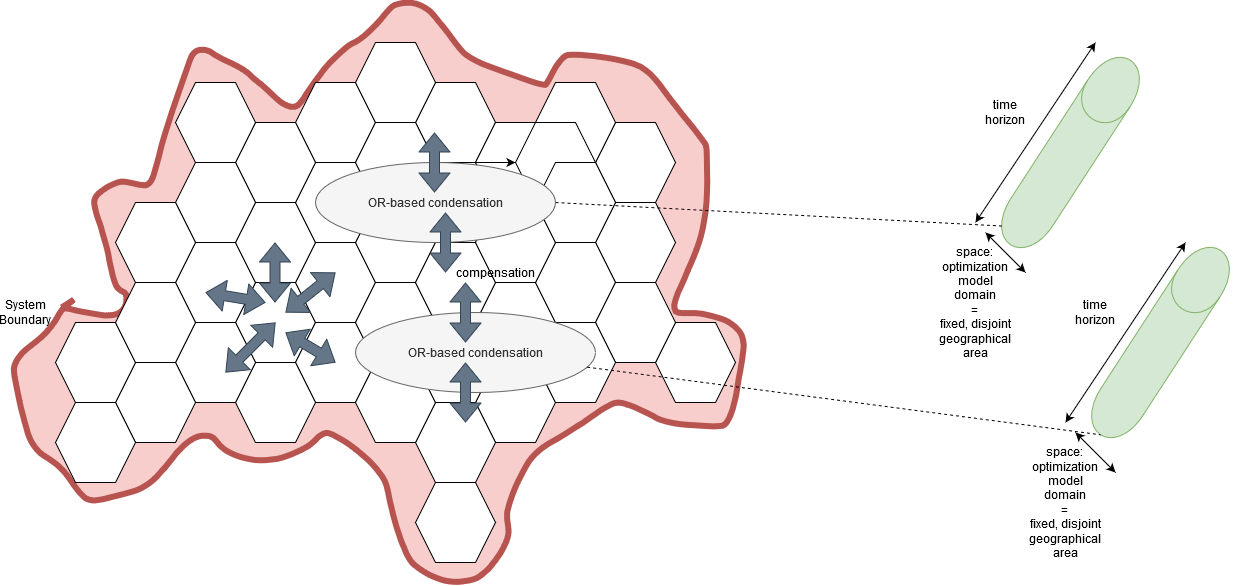
\includegraphics[width=0.9\textwidth]{introduction_compensation.png}
	\caption{}
	\label{fig:introduction_compensation}
\end{figure}
%
There is a common view of the current situation within system boundaries; the whole system is decomposed into disjoint geographic cells of responsibility. Most of them are handled by humans: human dispatchers have a view of the full system and can communicate through structured (e.g. IT system of incident messages) or informal ways (e.g. phone call with station managers or locomotive drivers). There are only a few condensation areas \cite{caimi2009} (in bottleneck areas such as merging areas in front of large stations or tunnels) that are operated through automatic systems. Between these areas, trains need to be able to compensate: if trains are reordered, these decisions must be taken into account in the neighboring areas.





\subsection{Research Approach: Decomposition in Space and Time}
Physical railway infrastructure is expensive in building and maintenance \cite{sr40programm}.
Therefore, the existing infrastructure capacity should be exploited as best as possible.
As the number of trains operating increases and condensation areas increase in number and size, it will become increasingly difficult to compensate for decisions taken within condensation zones or to define restrictions that keep the effects on the neighboring compensation zones as predictable as possible.

We will argue that
\begin{description}
\item [H2] it is possible to predict the affected time-space, either from the problem structure or from historic data (see below, Section~\ref{subec:H2});
\item [H1] such a prediction allows for a speed-up of the OR model (see below, Section~\ref{subec:H1}).
\end{description}



To tackle this problem, our approach is to combine Operations Research and Domain-specific Learning to get the best of both worlds: an "Oracle" is able to predict the "impact" of a delay, with or without a knowledge base learnt by training; we hope the Oracle could predict which trains and which departures are or could be affected by the delay based on past decisions. This piece of information from the Oracle then helps the solver to constrain the search space or at least drive its search more efficiently (driving the branching process).

This approach is shown in Figure~\ref{fig:introduction_time_space}:
%
\begin{figure}[ht]
	\centering
  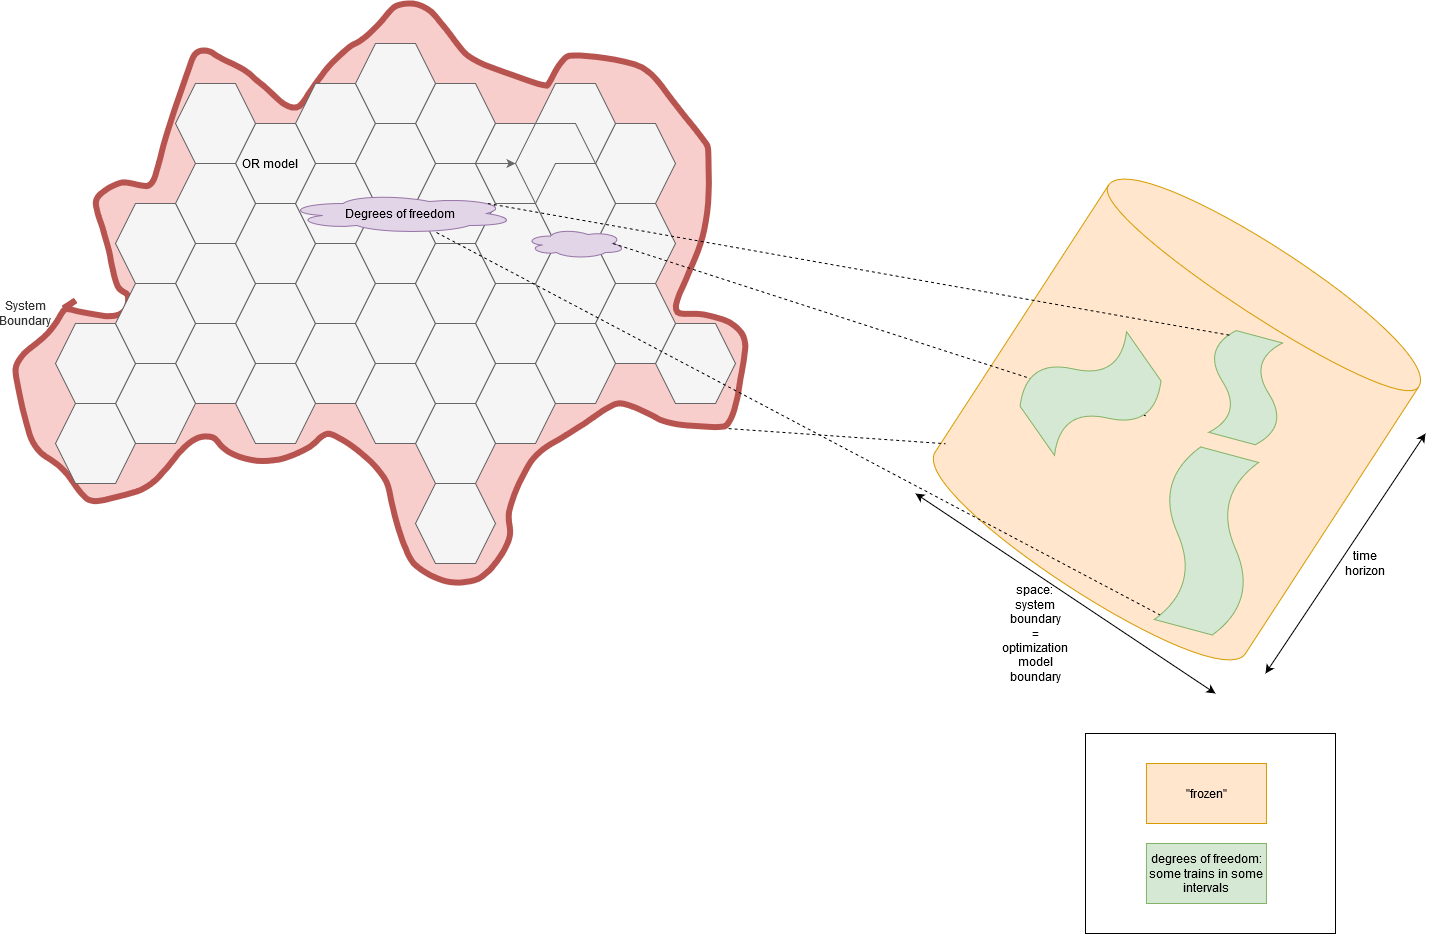
\includegraphics[width=0.9\textwidth]{introduction_time_space.png}
	\caption{}
	\label{fig:introduction_time_space}
\end{figure}
the Oracle predicts restrictions in time and space, which are passed to the solver.

\subsection{Research Approach: a Synthetic Playground}
We now give a short introduction to our playground implementation (G4) and its limitation with respect to real-world features.

\begin{description}
\item[Synthetic Infrastructure and Simplified Resource Model] \cite{aicrowdFLATland}
: Generator, no shared occupation
\item[Synthetic Timetable]
        Every train has one single source and target, no intermediate stations
        Every train has a constant speed (may be different from train to train)
        no cycles in the schedule
        schedule is generated to minimize sum of travel times satisfying an arbitrary upper bound → might be unrealistic
        no time reserves (no catching up)
        no distinction between published timetable and operational schedule (the published timetable imposes
        no connections or vehicle tours (turnrounds)
        no stops
        simplified train dynamics
\item[Synthetic route alternatives]
        10 shortest paths (in reality, in particular in the case of disturbances affecting a whole are, we might need a different scheme knowing the parts that cannot be taken)
\item[Simple Disturbance Model]:  one train stopped for d discrete time steps at time t; in reality, the delay might not be known or only probabilities can be assumed.
    In reality, update information comes in batches and we would need to consider multiple delays in the same update interval
\end{description}


\subsubsection{Hypothesis 1}\label{subec:H1}
show speed-up in at least one implementation
\subsubsection{Hypothesis 2}\label{subec:H2}
show some ideas, show why space and time


\section{Show Pipeline H1}
        Infrastructure generation
            Assumption and difference to real world
            Limitations
        Schedule and Malfunction Generation
            Stochastic Model
            Schedule cost function and link to real world
        Generic Solver Model ("ScheduleProblemDescription", mathematical ASP model)
        Re-scheduling Full and Delta ("ScheduleProblemDescription" in these cases with pseudo-code)
\section{Ideas H2}
        Heuristic ideas
        ML Ideas
\section{Discussion: show links to}
        ML
        delay propagation / recourse
        simulation
        OR / heuristics
        decomposition approaches
\section{Results H1}
\section{Early Results H2}



\bibliographystyle{unsrt}
\bibliography{biblio}

\end{document}






\section{Introduction}
Here we describe the Re-Scheduling problem.

Switzerland has a dense railway network with both freight and passenger trains running on the same infrastructure. More than 1.2 million people use trains on a daily basis. In Railway Operations, the operational schedule has to be continually re-computed because of many smaller and larger delays that arise during operations. Not all of those can be absorbed by extra times in the schedule, and if the delay has an impact on other trains, decisions on re-ordering or re-routing trains have to be taken to derive a new feasible operational plan. The industry state of the art is that delay propagation is efficiently re-computed by online IT systems. Conflicts, however, have to be most often resolved by humans by explicitly deciding on re-ordering or re-routing based on their experience. Because of the massive combinatorial complexity of these microscopic models, Operations Research models are currently only applied in very restricted, highly condensed areas for re-ordering decisions but do not consider routing alternatives.
Research Approach

To tackle this problem, our approach is to combine Operations Research and Machine Learning to get the best of both worlds: a Graph Neural Network acts as an Oracle for Operations Research by learning a heuristic that predicts the "impact" of a delay; we hope the Oracle could predict which trains and which departures are or could be affected by the delay based on past decisions. This piece of information from the oracle then helps the (MILP or CP) solver to constrain the search space or at least drive its search more efficiently (driving the branching process). We hope that Graph Neural Networks are a natural way to represent the graph structure of railway networks.

Our considerations are based on the Re-Scheduling Effects Model of Figure~\ref{fig:EffectsModel}:
the Operational Schedule is based on being informed about delays and the schedule communicated to customers. Interventions may be redefine the allowed speeds per location or per train, the available routes, the connections to be kept or dropped and trains to be added or dropped. Interventions may be directly based on events happening in reality or based on the current network status aggregated from past events.
%
Events from reality are interpreted when lead to a difference to the Operational Schedule.
%
\begin{figure}[ht]
	\centering
  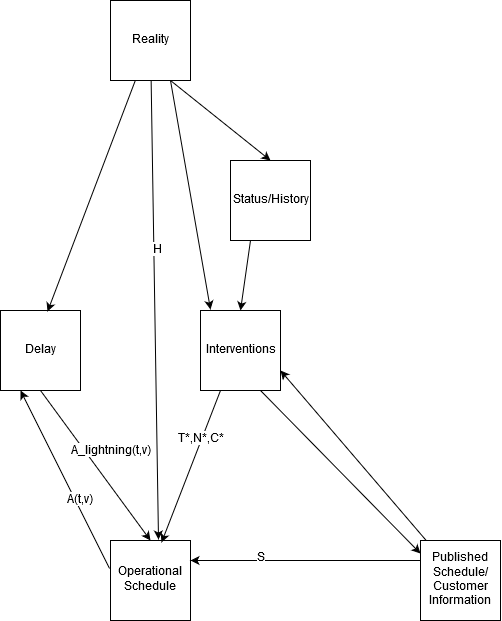
\includegraphics[width=0.7\textwidth]{Wirkungsmodell.png}
	\caption{Re-Scheduling Effects Model. Arrows represent logical dependencies. The symbols on the arrows are those used in the formal problem description later on.}
	\label{fig:EffectsModel}
\end{figure}
\section{Related Work}

TODO Related Work. How does it relate to \cite{DBLP:journals/corr/abs-1807-11876}?
TODO Other different approaches: Benders-like decomposition and loop, generate-and-verify-loop


\section{Methodology}
Here we describe the three hypotheses and the pipeline.

\subsection{3 Hypotheses, one building on the previous}
\begin{description}
\item[Hypothesis 1] We can compute good recourse actions, i.e., an adapted plan within a small fraction of the full solution time if all variables are fixed, except those related to services that are affected by the disruption implicitly or explicitly.
\item[Hypothesis 2] Machine learning can predict services that are affected by disruptions implicitly or explicitly with respect to a fixed infrastructure and a fixed basic (published) schedule, without the intention of model training to generalize over infrastructures nor completely new timetable concepts.
\item[Hypothesis 3] If hypothesis 2 is true, in addition, machine learning can predict the state of the system in the next time period after re-scheduling.
\end{description}

\subsection{A General Framework}
Our approach can be seen as a general framework with the following ingredients:
\begin{description}
\item[Detailed Model] We have a model  that reflects the detailed  view but which cannot be applied because it would be intractable. A detailed model acts at the operational and could be produced in reality if no further delays or disruptions happen; it not only works at the more imprecise tactical level. Formally, the detailed model is a deterministic solver that produces an operational plan ${\bf y}^*({\bf x})$ for a problem ${\bf x}$.
\item[Oracle] An Oracle predicts relevant parts of the solution such that the detailed exact model becomes tractable if we complement it by the informed guess by the Oracle.
Formally, an Oracle ${\cal O}$ produces an enhanced input ${\cal O}({\bf x})$ such that ${\bf y}^*({\cal O}({\bf x}))$ can be computed more efficiently.
\item[Simulation] Verifying an Oracle in the real world is often too expensive, either in financial terms or because of legal or other risk issues. Simulation allows us to train and verify the Oracle without having to run those risks. More formally, a simulation produces realistic inputs ${\bf x}$ (following the same distribution).
\end{description}



\subsection{Pipeline for Verification of Hypothesis 1}
Input generation
Step
Generate infrastructure
Generate schedule
Generate disturbance
Full Schedule (w/o disturbance)
Hypothesis Validation

How big is the speed up if we know Delta?
Step
Re-Scheduling full w/o restrictions
Determine Delta w.r. to Full Schedule
Re-Scheduling Delta



\section{Formal Problem Definition}
\subsection{FLATland Formal Definition}
Gridworld and Semantics. I'd like to formalize this. I think it would be worth to describe the FLATland semantics (synchronization, entering Grid, malfunctions, speed model). This will help us to generalize/abstract.


\subsection{Scheduling Problem}
Our formulation is based on \cite{DBLP:conf/lpnmr/AbelsJOSTW19}, but we slightly modify it in order to make the equivalence of microscopic halting sections explicit in the mathematical formulation. We will need this explicit property in the definition the Re-Scheduling Problem.\footnote{TODO: consistency of connections is not enforced - do we need it?} The naming is based on \cite{crowdAISBB}.


A \emph{Scheduling Problem} is a triple $(N,T,C)$ consisting of
\begin{itemize}
    \item a \emph{Railway Network} $N=(V,E,R,m,a,b)$ where
    \begin{itemize}
        \item \emph{global route graph} $(V,E)$, which  is a directed graph; the edges are also called \emph{route sections}
        \item $R$ is a set of resources
        \item \emph{minimum travel times} per route section $m: E \to \NNN$
        \item \emph{resource allocations} on route sections $a: R \to 2^E$
        \item \emph{blocking or release times} per resource $R\to \NNN$

    \end{itemize}
    \item \emph{trains} T of the form $T\ni t = (V^t,E^t,e^t, l^t,w^t)$ where
    \begin{itemize}
        \item \emph{route graph} $(V^t,E^t)$ is an acyclic sub-graph of $(V,E)$
        \item \emph{earliest passing time} of train $t$ at a vertex: $e^t: V^t \to \NNN$
        \item \emph{latest passing time} of train $t$ at a vertex $l^t: V^t \to \NNN$
        \item \emph{waiting times} of train $t$ on edge $w^t: E^t \to \NNN$
        \item a partition $W^t=\{W_1^t,\ldots,W_n^t\} \subseteq 2^{E^t}$ of equivalent microscopic edges such that every path  $p=(v_0,\ldots,v_k) \subseteq V^t$ for $(v_i,v_{i+1})\in E^t$ for $i=1,\ldots,n-1$ \footnote{We use the following notation: $(v_0,\ldots,v_n)\subseteq V^t$ denotes an ordered subset of elements of $V^t$. TODO: Should we formally introduced the set of paths in $V^t$, relating to $E^t$ to simplify notation?} such that $in(v_0)=0$ and $out(v_n)=0$ contains exactly one element of each partitioning element $W_i$, $i=1,...,n$ (i.e. there is exactly one edge $w(W_i^t)=(v_j,v_{j+1})\in E^t$ for $W_i^t \in W$ and  $v_j,v_{j+1}\in p$ and such that all $w(W_i^t)$ are different (i.e. $w$ is injective)).
    \end{itemize}
    \item \emph{connections} $C\subseteq T \times E \times T \times E \times \NNN$ such that $(t_1,e_1,t_2,e_2,c)\in C \implies e_1 \in E^{t_1}, e_2 \in E^{t_2}$
\end{itemize}
Note that $(V,E)$ needs not be connected, i.e. each train may have its own (disjoint) route sub-graph, which is linked to other trains' route graph only through shared resources in $R$, and the union of of all train-specific route graphs needs not cover $(V,E)$.
Notice that the some consistency conditions of the real-world problem are not part of this formal definition, for instance we would have to ensure that every path can produce the commercial stops on different platform tracks.

A solution $(P,A)$ of the Scheduling Problem consists of the
\begin{itemize}
    \item the selected paths $P: T \to 2^V$ where $p(t)=(t_1,\ldots,t_n)\subseteq V^t$ (we use $\ell(p(t))=n$ for the length of the path) is an ordered set satisfying
        \begin{equation}
            (v_i, v_{i+1})\in E^t\textrm{  for }i\in\{1,\ldots,n-1\} \label{eq:path_consistency}
        \end{equation}
        \begin{equation}
            in(v_1)=0\textrm{ and } out(v_n)=0 \label{eq:start_and_target_node}
        \end{equation}
        where $in:V\to\NNN$ and $out:V\to\NNN$ associate in and out degrees of vertices.
    \item partial allocation $A: T\times V \to \NNN$ where $A(t,v)$ is defined for $v\in P(t)$ satisfying
        \begin{equation}
            A(t,v) \geq e^t(v)\textrm { for } v \in P(t) \label{eq:earliest_requirement}
        \end{equation}
        \begin{equation}
             A(t,v) \leq l^t(v)\textrm { for } v \in P(t) \label{eq:latest_requirement}\\
        \end{equation}
        \begin{equation}
             A(t,v_i) + m((v_i,v_{i+1}) + w^t((v_i,v_{i+1})) \leq A(t,v_{i+1}) \label{eq:minimum_running_time_requirement}
        \end{equation}
        \begin{eqnarray}
             A(t_1, v^\prime) +b(r)\leq A(t_2, u) \xor A(t_2, u^\prime) +b(r) \leq A(t_1, v) \nonumber\\
             \textrm { for } v,v^\prime in  \in P(t_1), u,u^\prime \in P(t_2), (v,v^\prime),(u,u^\prime)\in a(r)
             \label{eq:mutual_resource_allocation_requirement}
        \end{eqnarray}
        (where $\xor$ denotes exclusive or)
        \begin{equation}
             A(t_1, v) +c\leq A(t_2, u) \textrm{ for }(t_1,(v,v^\prime),t_2,(u,u^\prime),c) \in C\label{eq:connection_requirement}
        \end{equation}
\end{itemize}

\subsection{FLATland as Scheduling Problem}
How are the route graphs derived from FLATland in general?


\subsection{Commercial and Operational Schedule}
The result of the above (offline) Scheduling Approach is a conflict-free (microscopic) solution. We therefore call it an \emph{Operational Schedule}.
If everything runs smoothly, it contains all the information required to run trains.

What we publish to customers needs not be as details and may not even be conflict-free in the microscopic sense. For instance, we might publish two trains to start at the same time and decide online which one goes first whichever is ready first.
Formally, given an Operational Schedule $(P,A)$,
a \emph{Commercial or Published Schedule} captures the elements published to consumers\footnote{TODO: Should the connections be part of the Commercial Schedule as well?}. Formally,
\begin{itemize}
    \item $S(t,v)$ is the published schedule, partially defined for $v_{i+1} \in P(t)=(v_1,\ldots,v_n)$ where $w^t(v_i)>0$ and satisfying $S(t,v)\leq A(t,v)$ and $S(t,v_j) \leq S(t,v_k)$ for $j<k$ and $v_j,v_k \in P(t)$
\end{itemize}
i.e. we allow for conflicts in the commercial schedule, but guarantee that we never depart earlier than published in $S$.



\subsection{Re-Scheduling Problem}
Given a
\begin{itemize}
    \item Operational Schedule $(P,A)$,
    \item Commercial Schedule $S$
    \item the current time $H \in \NNN$
    \item operational interventions in the form of a scheduling problem $(N^*,T^*, C^*)$
    \item an event $A^\lightning(t^\lightning,v^\lightning)\geq H$, $A^\lightning(t,v)\not=A^(t,v)$, $A(t,v) \geq H$
\end{itemize}
The interpretation of $H$ is that we have received all information up to $H$, i.e. all times  $A(v,t) \leq H$ are fixed, i.e. they are already included included in our current operational schedule (either because they worked according to our initial plan or because we have already updated our current operational schedule). We require $A^\lightning(t,v) \geq H$; the interpretation is that $A^\lightning(t^t\lightning,v^\lightning)$ is a prognosis when train $t$ will pass at $v$ for $A(t,v)\geq H$.
Examples:
\begin{itemize}
    \item If $A^\lightning(t^\lightning,v^\lightning)=H$ and we know that we will be ready only later on at $A^\lightning(t^\lightning,v^\lightning)\not=A^(t^\lightning,v^\lightning)$, $A(t,v) \geq H$.
    \item If $A(t^\lightning,v^\lightning)>H$, we might know that we will be ready earlier at $A^\lightning(t^\lightning,v^\lightning) < A(t^\lightning,v^\lightning)$
\end{itemize}
A \emph{Re-Scheduling Oracle} is a pair $(F_1,F_2)$
\begin{itemize}
    \item $F_1\subseteq T^*$ and $\GG(t)=(\bar{V}^t,\bar{E}^t)$ is an acyclic connected sub-graph of $(V,E)$ for $t \in F_1$
    \item $F_2\subseteq T^*\times V$ where $(t,v)\in F_2 \implies A(t,v)\geq H, v\in P(t), t\not\in F_1$.
    \item  $T(F_2)\cap F_1 = \emptyset$ where $T(F_2) = \{ t: (t,v) \in F_2)$
\end{itemize}
The situation is depicted in Figure~\ref{fig:ReSchedulingFlexi}: there are trains with no flexibility, trains with time flexibility and trains with routing and time flexibility. Notice that the route graphs $\GG(t)$ may grow or shrink with respect to the initial Scheduling Problem, i.e. we may allow for route alternatives that were not allowed for planning. We even allow for trains and connections to be added or dropped.
%
\begin{figure}[ht]
	\centering
  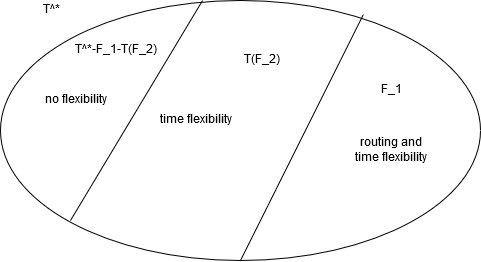
\includegraphics[width=0.7\textwidth]{flexibility.png}
	\caption{Degrees of flexibility for the Re-Scheduling-Problem.}
	\label{fig:ReSchedulingFlexi}
\end{figure}



A Solution $(\bar{P},\bar{A})$ of the Re-Scheduling Problem is a solution to the Scheduling Problem $(N^*,T^*,C^*)$, further satisfying
\begin{equation}
    \bar{P}(t) = P(t) \textrm{ for } t \not \in F_1,\label{eq:freedom_alternative_paths}
\end{equation}
\begin{equation}
    \bar{A}(t,v) = A(t,v) \textrm{ for } t \not \in F_1, t \not \in T(F_2), \label{eq:freedom_times_only}
\end{equation}
\begin{equation}
    \bar{A}(t,v^\prime) \geq S(t,v) \textrm { for all } S(t,v) \textrm{ and some } v^\prime \in W(_,v) \label{eq:respect_commercial_schedule}
\end{equation}
as well as equations (\ref{eq:path_consistency}),
(\ref{eq:start_and_target_node}),
(\ref{eq:minimum_running_time_requirement}),
(\ref{eq:mutual_resource_allocation_requirement}),
(\ref{eq:connection_requirement}) above and minimizing
\begin{equation}
    \sum_{(t,v) \in \dom(S)} \bar{A}(t,v) -S(t,v).
\end{equation}
The Re-Scheduling Oracle defines the degrees of freedom on two levels, allowing path alternatives for trains $t\in F_1$ and allowing for modified departure times for the departures in $F_2$, but we require trains to respect the Commercial Schedule, i.e. we do not allow for trains or stops to be dropped.

\section{Results Hypothesis 1}

\subsection{Implementation Details}
k shortest paths, constraints in the model above, best-case Oracle

Our setting for Re-Scheduling for step XX in \cite{DBLP:journals/corr/abs-1807-11876}:
\begin{itemize}
    \item $N^*=N$
    \item $T$ = shortest path or all routes
    \item $C^*=C$
    \item $F_1$, $F_2$?
\end{itemize}{}

\section{Results Hypothesis 2}
\subsection{DL approaches}

\subsubsection{Graph-based Neighborhood Search (GNN)}
Approach Christian B. + Mayra

\subsubsection{Probabilistic Schedule (GNN)}
Erik

\subsubsection{Reinforcement Learning}
Erik with Jakab/Levent?

\subsection{Heuristics Oracle}

\subsubsection{Deadlock Avoidance}
Extending Adrian's Deadlock-Avoidance Algorithm? Christian E. and Adrian?



\subsubsection{Job Insertion}
Blocking Job-Shop-Scheduling Fribourg (Reinhard Bürgy)? Christian E. with Reinhard?

\subsection{Exploiting the Oracle in OR}
Christian E.

\section{Conclusion}
What have we achieved?

\section{Future Work}
Describe the Research Plan and the Challenge for other Researcher.


\section*{To Discuss}
\begin{itemize}
    \item definition of operational schedule should be independent of the scheduling problem based on time windows, definition is not very readable
    \item - not use $t$ for train but for time? Confusing for physicists....
    \item use real numbers for event times
    \item which cost function (classes) do we want to consider?
    \item use different mathematical problem formulation (alternative/disjunctive graph job shop scheduling,....?)
    \item Further Research: not only consider isolated events?
    \item Further Research: drop trains, drop halts, ...
    \item Further Research distributions or time windows as prognosis not only fixed event time
\end{itemize}


\bibliographystyle{unsrt}
\bibliography{biblio}

\end{document}
